\chapter*{End-of-Semester Progress Report} % Using chapter* for unnumbered main title
\label{chap:progress_report}

\section*{Brief Summary}
\label{sec:progress_summary}
This semester's development for the SpotOn project has focused on two primary streams: establishing a robust MLOps pipeline and designing a modular backend system. Significant progress has been made in the MLOps domain, including comprehensive experimentation with person detection models using MLflow, implementation of model training and explainability techniques, and initial design for model deployment as a service. Key AI models like Faster R-CNN were fine-tuned and evaluated on the MTMMC dataset.

Concurrently, the backend system architecture has been designed to support retrospective video analysis. This includes defining API endpoints with FastAPI, WebSocket communication protocols for real-time metadata streaming, and a data processing pipeline that integrates AI components for detection, tracking, re-identification, and spatial mapping. The design emphasizes modularity using service layers and design patterns like Strategy and Repository to ensure scalability and maintainability for future development.

In parallel, frontend development has successfully established WebSocket-based communication to receive processed data streams from the backend. This enables the user interface to dynamically display tracking information and analytical results, providing users with a real-time visual representation of the SpotOn system's capabilities.


\section*{Detailed Development Description}
\label{sec:progress_detailed_development}

\subsection*{MLOps Progress}
\label{subsec:progress_mlops}
The MLOps efforts have concentrated on building a repeatable and traceable workflow for developing and evaluating the AI components of SpotOn.

\subsubsection*{Key MLOps Developments and Designs:}
\begin{itemize}
    \item \textbf{ML Canvas Design:} A comprehensive ML Canvas was formulated to guide the AI system's development. It details the core problem of multi-camera tracking, input data requirements (primarily the MTMMC dataset from S3), the proposed processing approach (utilizing models like Faster R-CNN for detection, BotSort for tracking, and CLIP for Re-ID features), expected outputs (such as annotated video metadata for the UI, map visualizations, and historical data for TimescaleDB), and the criteria for evaluating success.
    
    \begin{figure}[!htb]
        \centering
        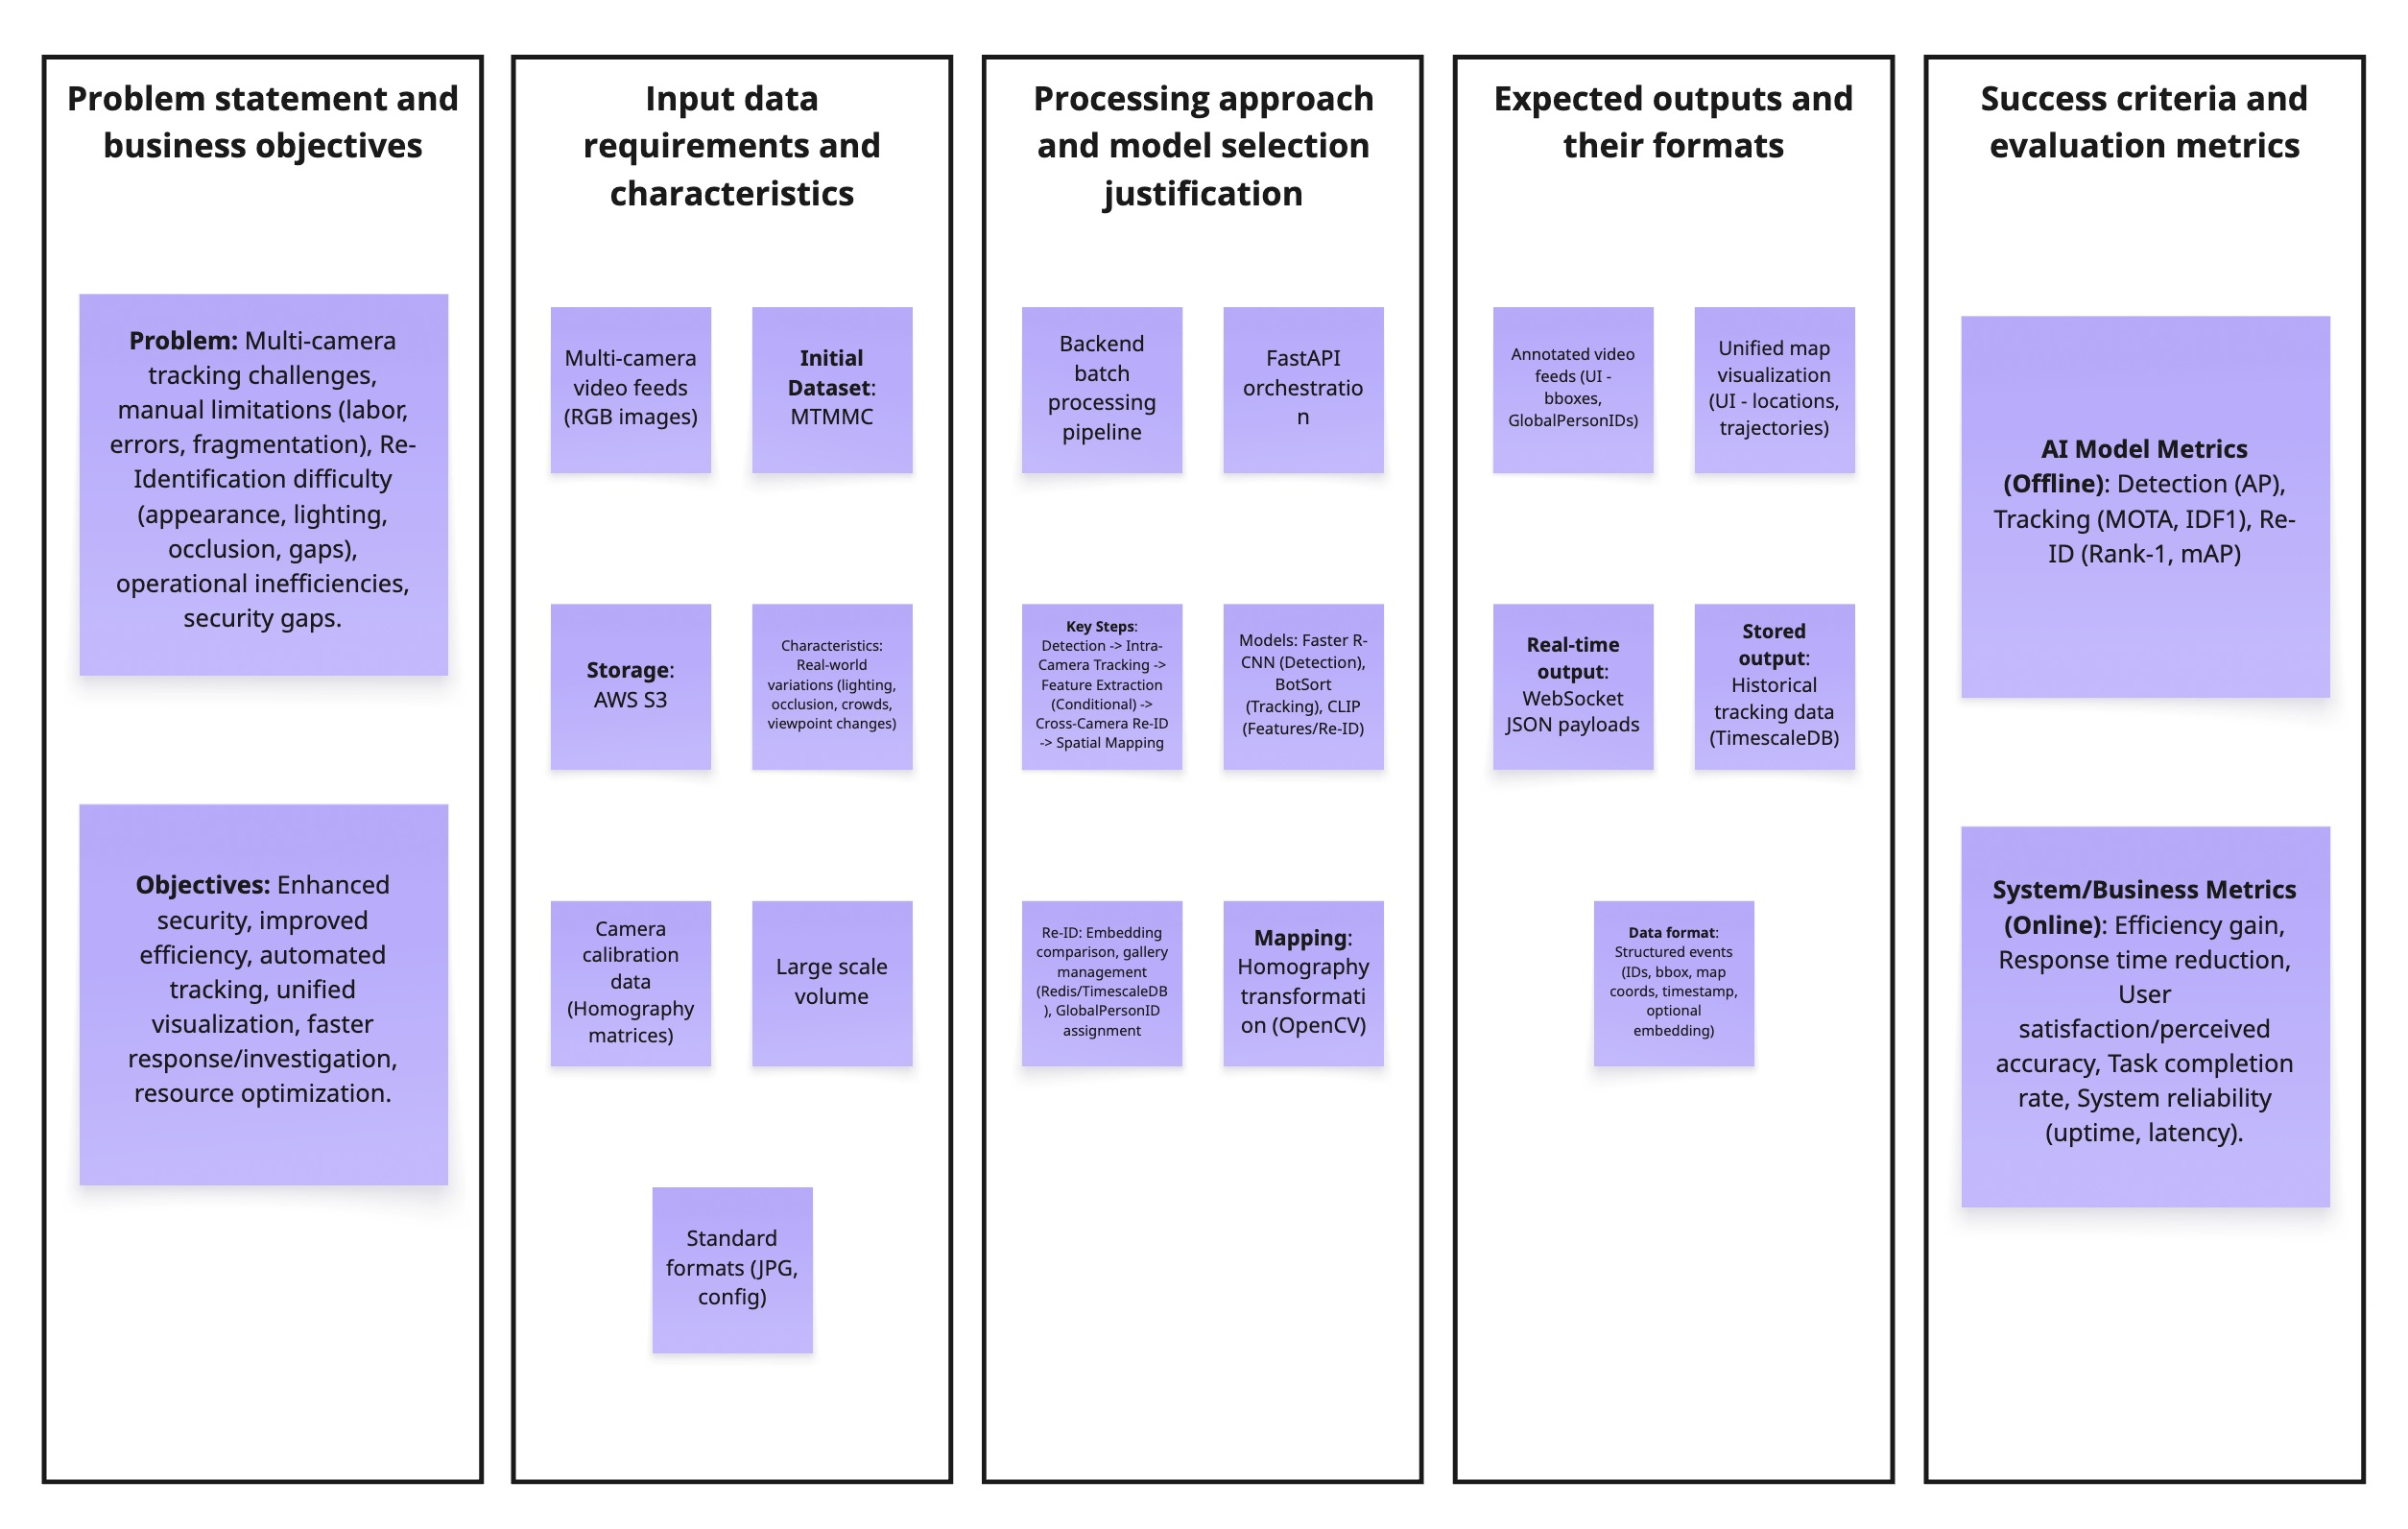
\includegraphics[width=0.8\textwidth]{progress/ml_canvas.jpg}
        \caption{Overview of the ML Canvas for SpotOn}
        \label{fig:progress_ml_canvas}
    \end{figure}
    
    From Figure \ref{fig:progress_ml_canvas}, the main components of the ML problem, data sources, processing steps, and evaluation metrics defined for SpotOn are visualized.

    \item \textbf{Model Training Implementation:} An end-to-end training pipeline for the Faster R-CNN person detection model was implemented using PyTorch and TorchVision. This pipeline encompasses initial data exploration of the MTMMC dataset, robust preprocessing steps (including image resizing, color conversion, normalization, and data augmentation techniques like random horizontal flipping), definition of the model architecture (ResNet-50 backbone with FPN), and modification of the classification head specifically for person detection. The training loop integrates MLflow for systematic experiment tracking and management. Furthermore, unit tests were developed to ensure the reliability of dataset loading mechanisms, metric calculation functions, and various utility components.
    \clearpage
    \begin{figure}[!htb]
        \centering
        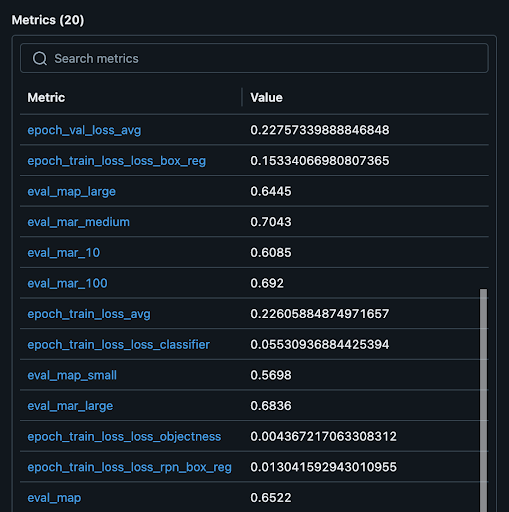
\includegraphics[width=0.8\textwidth]{progress/detection_metric.png}
        \caption{Sample MLflow Metrics from Faster R-CNN Training Runs}
        \label{fig:progress_mlflow_training_metrics}
    \end{figure}
    
    Figure \ref{fig:progress_mlflow_training_metrics} illustrates typical performance metrics, such as loss and mAP, tracked during the model training process, providing insights into learning progression.


    \item \textbf{Model Fairness Analysis:} A conceptual framework for analyzing and mitigating potential biases within the AI models was established. This involved identifying potential sources of bias in the MTMMC training data (such as demographic imbalances or environmental variations) and outlining strategies for fairness metric calculation (e.g., comparing Re-Identification accuracy disparities across different proxy groups defined by observable characteristics like lighting conditions or occlusion levels). Mitigation approaches, including data-based techniques (targeted augmentation, re-sampling), model-based methods (adversarial debiasing, fairness regularization), and post-processing adjustments, were also considered.

    \item \textbf{Model Versioning and Comparative Experimentation:} MLflow was employed as a central tool for versioning AI models and conducting systematic comparative experiments. Several person detection architectures, including Faster R-CNN, RT-DETR variants, and YOLO, were evaluated. Key parameters (model name, type, weights path) and performance metrics (mAP, FPS, total person detections) were meticulously logged for each experimental run. This data-driven approach led to the selection of Faster R-CNN as the baseline person detection model, primarily due to its strong performance on medium-sized objects, higher overall recall, and observed qualitative stability.

    \begin{figure}[!htb]
        \centering
        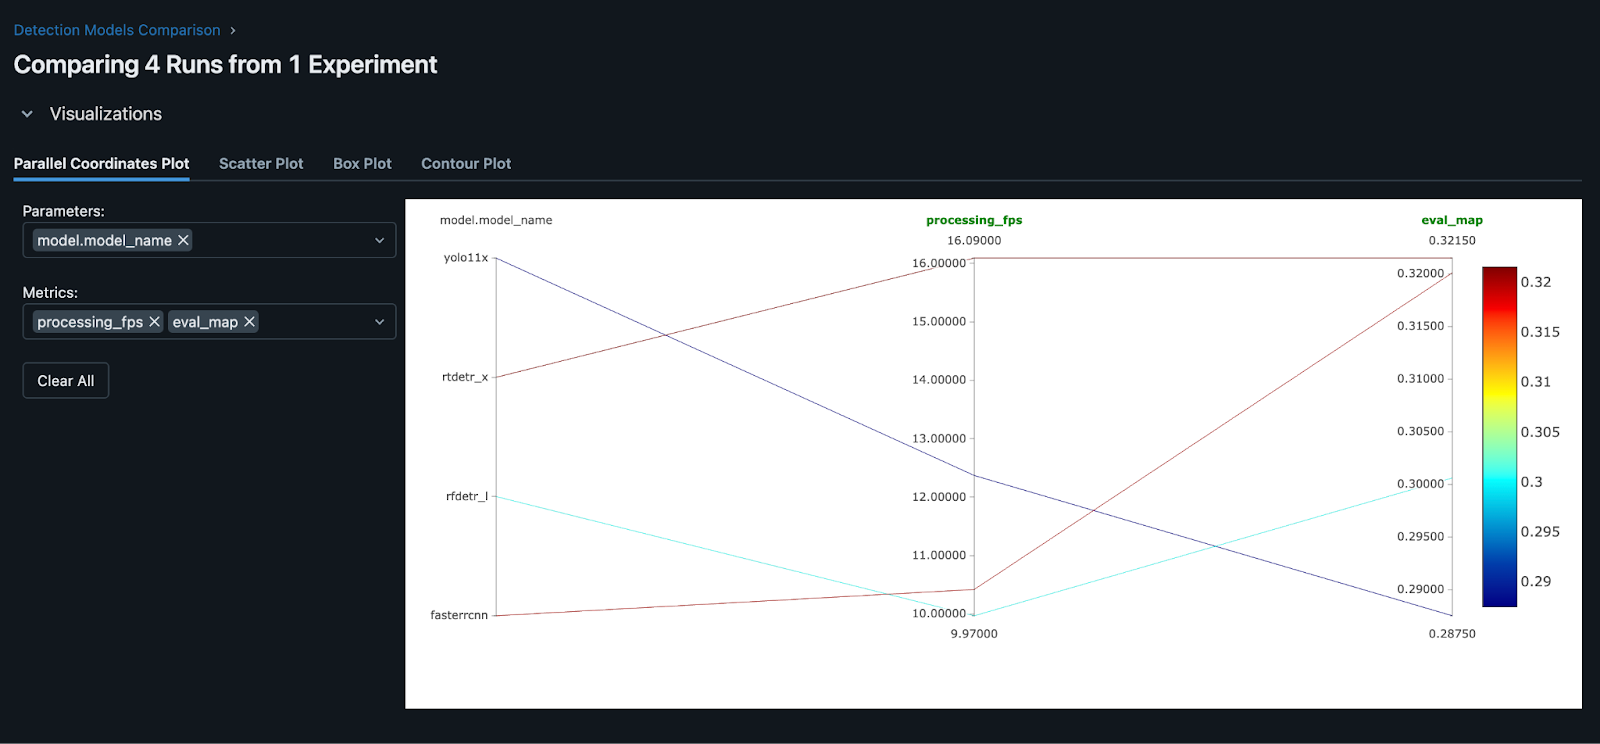
\includegraphics[width=0.8\textwidth]{progress/detection_comparison.png}
        \caption{MLflow Interface Showing Detection Model Comparison}
        \label{fig:progress_mlflow_model_comparison}
    \end{figure}
    
    As depicted in Figure \ref{fig:progress_mlflow_model_comparison}, the MLflow interface facilitates a side-by-side comparison of different models based on key performance indicators logged during experimentation.

    \item \textbf{Model Explainability Techniques:} To enhance transparency and trustworthiness, Grad-CAM (Gradient-weighted Class Activation Mapping) was implemented using the Captum library. This technique generates visual heatmaps that highlight the specific image regions most influential in the Faster R-CNN model's decision-making process for person detection, offering insights into its internal workings.
    
    \begin{figure}[!htb]
        \centering
        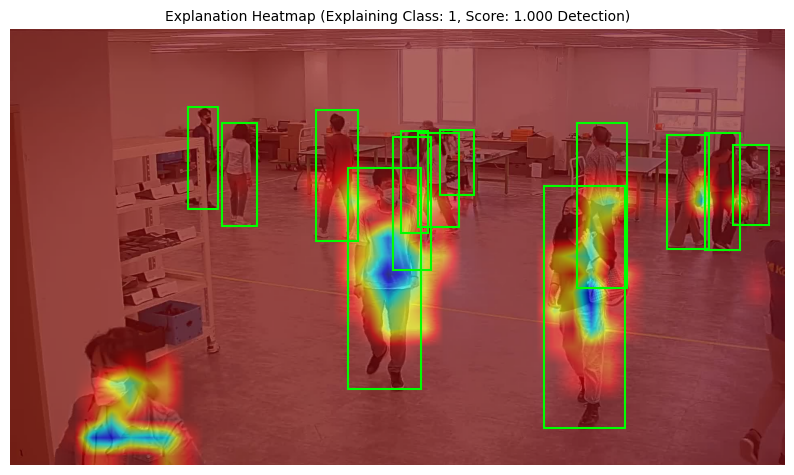
\includegraphics[width=0.7\textwidth]{progress/gradcam_example.png}
        \caption{Example of Grad-CAM Visualization for Person Detection}
        \label{fig:progress_gradcam_example}
    \end{figure}
    
    Figure \ref{fig:progress_gradcam_example} provides a visual example of how Grad-CAM highlights influential image regions for a person detection, aiding in understanding the model's focus.

    \item \textbf{Prediction Reasoning Mechanism:} Building upon the visual explanations, a mechanism was developed to generate human-understandable textual justifications for individual model predictions. This system combines the quantitative confidence score of a detection with qualitative insights from the Grad-CAM analysis, providing users with a clearer understanding of why a particular prediction was made.

    \item \textbf{Model Deployment as a Service Design:} The architectural design for deploying the trained AI models as a service was completed. This involves a backend API layer built with FastAPI, featuring documented RESTful endpoints for initiating and monitoring video processing tasks, and WebSocket endpoints for streaming real-time tracking metadata (bounding boxes, global IDs, map coordinates) to client applications. The functionality of this service-based deployment was validated using a Python-based test client simulating frontend interactions.
    
    \begin{figure}[!htb]
        \centering
        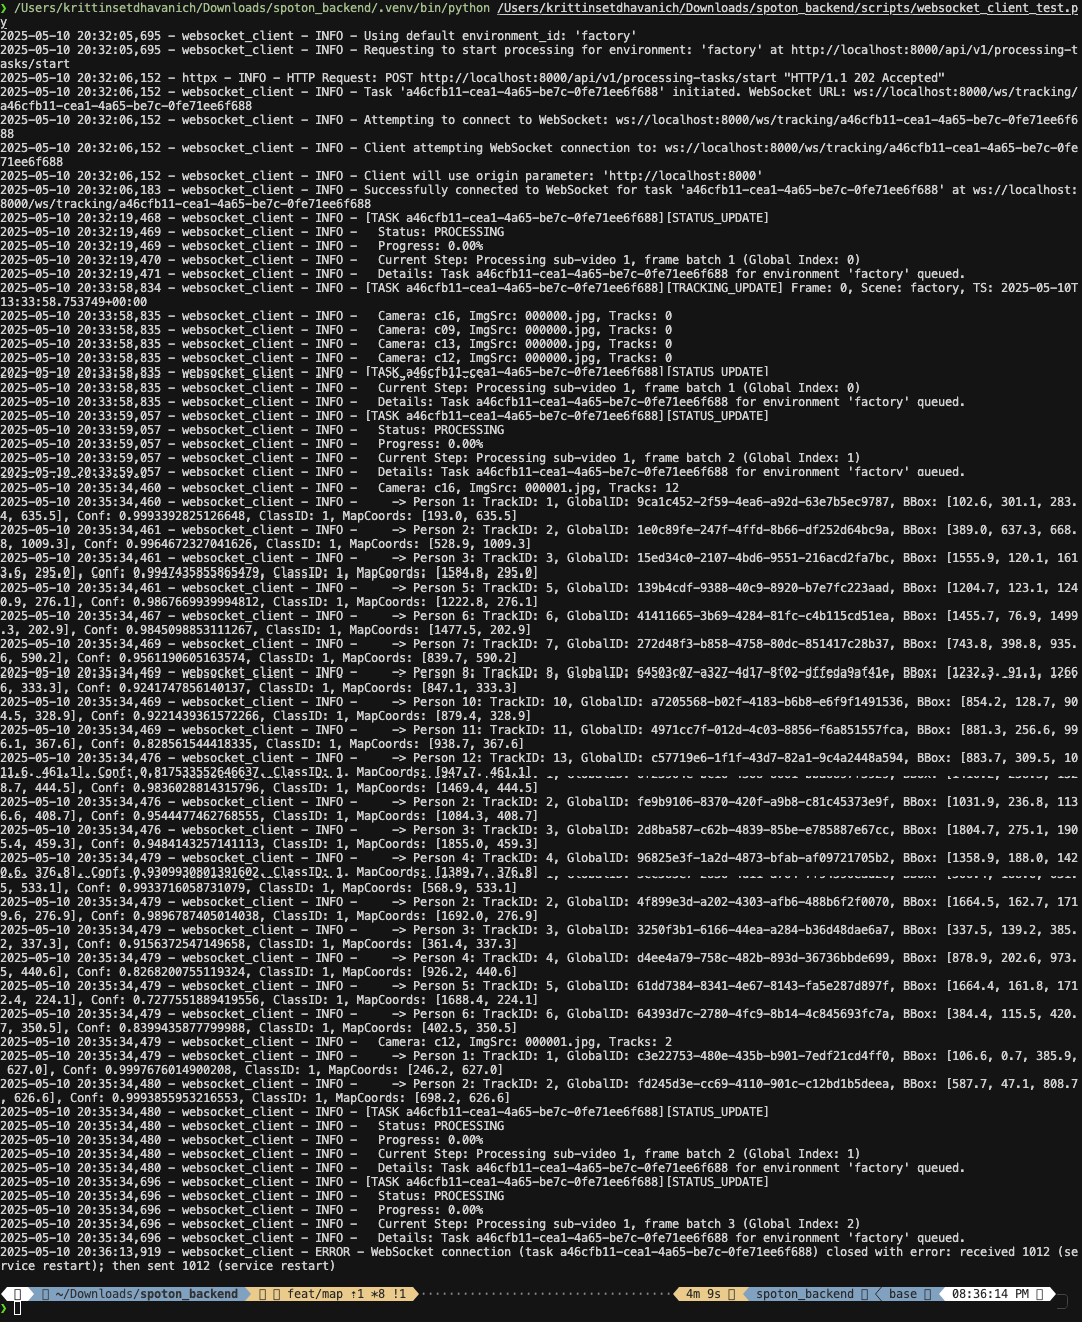
\includegraphics[width=0.9\textwidth]{progress/ws_server_log.png}
        \caption{Logs Demonstrating API and WebSocket Communication for Deployed AI Service}
        \label{fig:progress_api_logs}
    \end{figure}
    The logs presented in Figure \ref{fig:progress_api_logs} confirm the successful establishment and data exchange over API and WebSocket channels for the AI service prototype.
\end{itemize}

\clearpage

\subsubsection*{Experimental Results Summary (MLOps)}
\begin{itemize}
    \item \textbf{Faster R-CNN Initial Training:} An initial fine-tuning run on a 10\% subset of the MTMMC dataset for 5 epochs demonstrated the model's learning capability, achieving an overall mAP of 0.6522 and an mAP@0.50 of 0.8954. The proximity of training and validation losses suggested no significant overfitting during this preliminary phase.
    \item \textbf{Detection Model Comparison:}
        \begin{table}[!htb]
          \centering
          \caption{Key Performance Metrics from Detection Model Comparison}
          \label{tab:progress_model_comparison_summary}
          \begin{tabular}{@{}lcc@{}}
            \toprule
            Model Name & eval\_ap\_person & processing\_fps \\ \midrule
            {rtdetr\_x} & 0.322 & 16.09 \\
            {fasterrcnn\_resnet50} & 0.320 & 10.42 \\
            {rtdetr\_l} & 0.316 & 9.48 \\
            {yolo11x} & 0.297 & 11.66 \\ \bottomrule
          \end{tabular}%
        \end{table}
    
        Faster R-CNN (fasterrcnn\_resnet50) was selected as the baseline detection model. While RTDETR-X showed marginally higher overall mAP and speed, Faster R-CNN demonstrated superior performance on medium-sized objects, a significantly higher count of total person detections (indicating better recall), and greater qualitative stability with fewer observed Non-Maximal Suppression (NMS) issues in initial tests.
\end{itemize}

\subsubsection*{Datasets Acquired or Used (MLOps)}
The \textbf{MTMMC (Multi-Target Multi-Camera) dataset} has been the primary data source for training, validating, and testing the AI models. This dataset, collected from real-world campus and factory environments using 16 multi-modal cameras, provides diverse and challenging scenarios crucial for developing a robust multi-camera tracking system.

\subsection*{Exploratory Data Analysis (EDA) of the MTMMC Dataset}
\label{subsec:progress_eda}
A comprehensive Exploratory Data Analysis (EDA) was conducted on the MTMMC dataset to understand its characteristics, structure, and data quality. This analysis is pivotal for informing data preprocessing strategies, model selection, and evaluation methodologies.


\subsubsection*{EDA Process Overview}
An automated EDA pipeline was developed and executed. This pipeline performed several key steps:
\begin{enumerate}
    \item \textbf{Data Discovery:} Scanned the dataset to identify available scenes, cameras, image sequences, and ground truth files based on a predefined configuration.
    \item \textbf{Annotation Loading:} Parsed all relevant ground truth files to consolidate annotations.
    \item \textbf{Statistical Calculation:} Computed a wide range of descriptive statistics regarding object counts, bounding box characteristics, and track lengths.
    \item \textbf{Quality Assessment:} Performed checks for data integrity, such as frame count mismatches between image files and annotations, out-of-bounds bounding boxes, and consistency in image dimensions.
    \item \textbf{Visualization Generation:} Created plots to visualize key distributions and the effects of standard preprocessing steps.
\end{enumerate}
All derived metrics, parameters, and generated artifacts from the EDA process were systematically logged for traceability and review.

\subsubsection*{Key EDA Findings and Observations}
The EDA, conducted on a representative subset of the MTMMC dataset (including factory scene `s10` and campus scene `s47` with multiple cameras like `c01-c16`), yielded quantitative metrics and qualitative insights into the data's nature.

\begin{itemize}
    \item \textbf{Overall Dataset Scale Parameters:} The analyzed portion comprised multiple scenes and cameras, revealing tens of thousands of frame indices, hundreds of thousands of annotations, and over one hundred unique person identities. These high-level parameters are summarized in Figure \ref{fig:progress_eda_parameters_summary}.

    \begin{figure}[!htb]
        \centering
        \includegraphics[width=0.8\textwidth]{assets/progress/eda_parameters.png}
        \caption{Summary of Key Dataset Parameters from EDA}
        \label{fig:progress_eda_parameters_summary}
    \end{figure}
    
    From Figure \ref{fig:progress_eda_parameters_summary}, key parameters like the total number of scenes, cameras, frame indices discovered, total annotations, and unique object IDs are presented, providing a scope of the analyzed data.

    \item \textbf{Annotation Characteristics and Distributions:} Statistical analysis of annotations provided insights into object properties. This included distributions of bounding box heights (min $\approx$30, mean $\approx$190, max $>$1600 pixels), widths, and areas. The number of annotations per frame typically ranged from 1 to 28 (median $\approx$6). Track lengths for individuals also showed significant variation (min $\approx$7, median $\approx$400, max $>$7000 frames). These detailed statistical metrics are captured in Figure \ref{fig:progress_eda_metrics_summary}.
    \clearpage
    \begin{figure}[!htb]
        \centering
        % Placeholder for an image
        \includegraphics[width=0.8\textwidth]{assets/progress/eda_metrics.png}
        \caption{Summary of Detailed Statistical Metrics from EDA}
        \label{fig:progress_eda_metrics_summary}
    \end{figure}
    Figure \ref{fig:progress_eda_metrics_summary} displays a collection of statistical metrics derived from the dataset, such as the minimum, maximum, mean, and median values for bounding box dimensions (height, width, area), track lengths, and annotations per frame.
    \clearpage
    \item \textbf{Data Quality Insights:}
        \begin{itemize}
            \item \textit{Frame Count Mismatches:} Discrepancies were noted between the number of image files and the extent of ground truth frame indices (e.g., one sequence had 7362 images but GT up to frame 7171).
            \item \textit{Out-of-Bounds Annotations:} A substantial number of bounding boxes extended beyond image dimensions, indicating objects partially out of view or potential annotation inaccuracies.
            \item \textit{Image Dimension Consistency:} Sampled images within individual camera streams generally showed consistent dimensions (e.g., 1920x1080).
        \end{itemize}

\subsubsection*{Significance of EDA}
The EDA provided critical insights into the MTMMC dataset's scale, content distribution, and quality. This understanding is essential for robust data preprocessing (e.g., handling out-of-bounds boxes, normalizing varied object sizes), appropriate model selection, and designing effective training and evaluation strategies tailored to the dataset's specific challenges.

\clearpage
\subsection*{Backend System Design Progress}
\label{subsec:progress_backend}
The backend system has been designed to orchestrate the AI processing pipeline and serve data to the frontend. The design emphasizes a modular, service-oriented architecture. To provide context for the backend's role and its technological environment within the broader SpotOn project, the overall system architecture is first presented.

\begin{figure}[!htb]
    \centering
    \includegraphics[width=0.9\textwidth]{assets/progress/system_architecture.jpg}
    \caption{Project Architecture Overview}
    \label{fig:system_architecture}
\end{figure}
Figure \ref{fig:system_architecture} presents a high-level overview of the project's complete system architecture, outlining the principal technology stacks and interconnected components. This includes the Frontend (React, Zustand), Backend services (FastAPI, PyTorch, OpenCV, Ultralytics, BoxMOT), MLOps pipeline (MLflow, DagsHub), data sources (Amazon S3), data storage and caching mechanisms (Redis, TimescaleDB, PostgreSQL), deployment and infrastructure (Docker, Kubernetes, Nginx), and monitoring tools (Prometheus, Grafana). The backend, a central part of this architecture, is detailed further below, focusing on its internal modules and workflow.

\subsubsection*{Key Backend Modules and Components Designed (as per Spoton Backend Design.md):}
\begin{itemize}
    \item \textbf{Application Structure (`app/`):}
        \begin{itemize}
            \item `api/`: Defines FastAPI routers for versioned API endpoints (e.g., `/api/v1/processing\_tasks`, `/api/v1/analytics\_data`) and WebSocket management (`websockets.py`). Pydantic models in `schemas.py` ensure data validation.
            \item `core/`: Handles application configuration (`config.py` using Pydantic `BaseSettings`) and lifecycle events (`event\_handlers.py` for model loading/unloading).
            \item `models/`: Contains wrappers for AI models (Detector, Tracker, FeatureExtractor) implementing the Strategy Pattern (e.g., `FasterRCNNDetector`, `BotSortTracker` wrapping BoxMOT).
            \item `services/`: Encapsulates business logic. Key services include:
                \begin{itemize}
                    \item `PipelineOrchestratorService`: Manages the core processing pipeline.
                    \item `ReIDService`: Handles Re-ID logic and gallery management.
                    \item `StorageService`: Implements Repository/DAO pattern for S3, Redis, TimescaleDB.
                    \item `HomographyService`: Manages coordinate transformations.
                    \item `NotificationService`: Pushes updates via WebSockets.
                \end{itemize}
            \item `tasks/`: Contains logic for background processing, such as `FrameProcessorTask` for per-frame AI operations.
            \item `utils/`: Common utility functions.
            \item `main.py`: FastAPI application entry point.
            \item `dependencies.py`: FastAPI dependency injection setup.
        \end{itemize}
    \item \textbf{Core Technologies:} The backend specifically leverages Python, FastAPI, PyTorch, OpenCV, BoxMOT, Redis, TimescaleDB, and Docker for its operations.
    \item \textbf{Design Patterns:} Key design patterns employed include Strategy, Factory, Service Layer, Repository/DAO, Observer (conceptually via WebSockets), Pipeline (conceptual), and Dependency Injection.
    \item \textbf{Data Flow:} A detailed data flow for retrospective analysis of pre-split sub-videos from S3 has been defined. This covers task initiation, sub-video fetching and caching, frame-by-frame AI processing (detection, tracking, Re-ID), data storage in TimescaleDB, and real-time metadata updates to the client via WebSockets. The internal workflow orchestrating this data processing is visualized next.
\end{itemize}

\begin{figure}[!htb]
    \centering
    \includegraphics[width=0.9\textwidth]{assets/progress/backend_workflow.png}
    \caption{Backend workflow illustrating key internal components and interactions.}
    \label{fig:backend_workflow}
\end{figure}
Figure \ref{fig:backend_workflow} illustrates this internal backend data flow and the interaction of key services, such as the pipeline orchestrator and notification service. It also shows how these services interface with data stores like S3 and TimescaleDB, and manage client communication via REST APIs and WebSockets.

\clearpage 
\subsection*{Frontend Progress}
\label{subsec:progress_frontend}
Key UI components have been successfully implemented to provide users with a comprehensive view of the surveillance analytics. This includes:
\begin{itemize}
    \item \textbf{Multi-Camera Feed Display:} A module for displaying video streams or image sequences from selected cameras, often annotated with AI-driven insights like bounding boxes.
    \item \textbf{Interactive Map Visualization:} A component that renders a 2D map of the monitored environment, dynamically updated with the trajectories and current locations of tracked individuals.
    \item \textbf{Controls and Navigation:}  Standard UI elements for user interaction, such as selecting cameras, time ranges for analysis, and focusing on specific tracked entities.
\end{itemize}
The design philosophy has focused on intuitive data presentation, aiming to reduce cognitive load on the operator and enable quick assimilation of critical information.
Real-time Data Integration and Display:
A crucial achievement this semester has been the successful integration of the frontend with the backend system via WebSockets. The frontend is now capable of:
\begin{itemize}
    \item \textbf{Establishing and Maintaining WebSocket Connections:} Connecting to the backend WebSocket server to receive continuous data streams.
    \item \textbf{Receiving Processed Analytical Data:} Consuming structured data payloads from the backend, which include person detections (with bounding boxes), global person IDs, tracking updates (status, re-identifications), and map coordinates.
    \item \textbf{Dynamic UI Rendering:} Utilizing the received data to dynamically update all relevant UI components in real-time. This means that as the backend processes video feeds, the frontend reflects these changes immediately—bounding boxes appear on camera views, trajectories extend on the map, and statistics in the detail panels are updated.
\end{itemize}
This successful implementation ensures that users can observe the output of the AI-powered tracking and analysis pipeline as it happens, providing immediate visual feedback and enabling effective monitoring and retrospective analysis through the developed interface. The data is retrieved and displayed finely, laying a solid foundation for further feature enhancements and user experience refinements.
\begin{figure}[H]
    \centering
    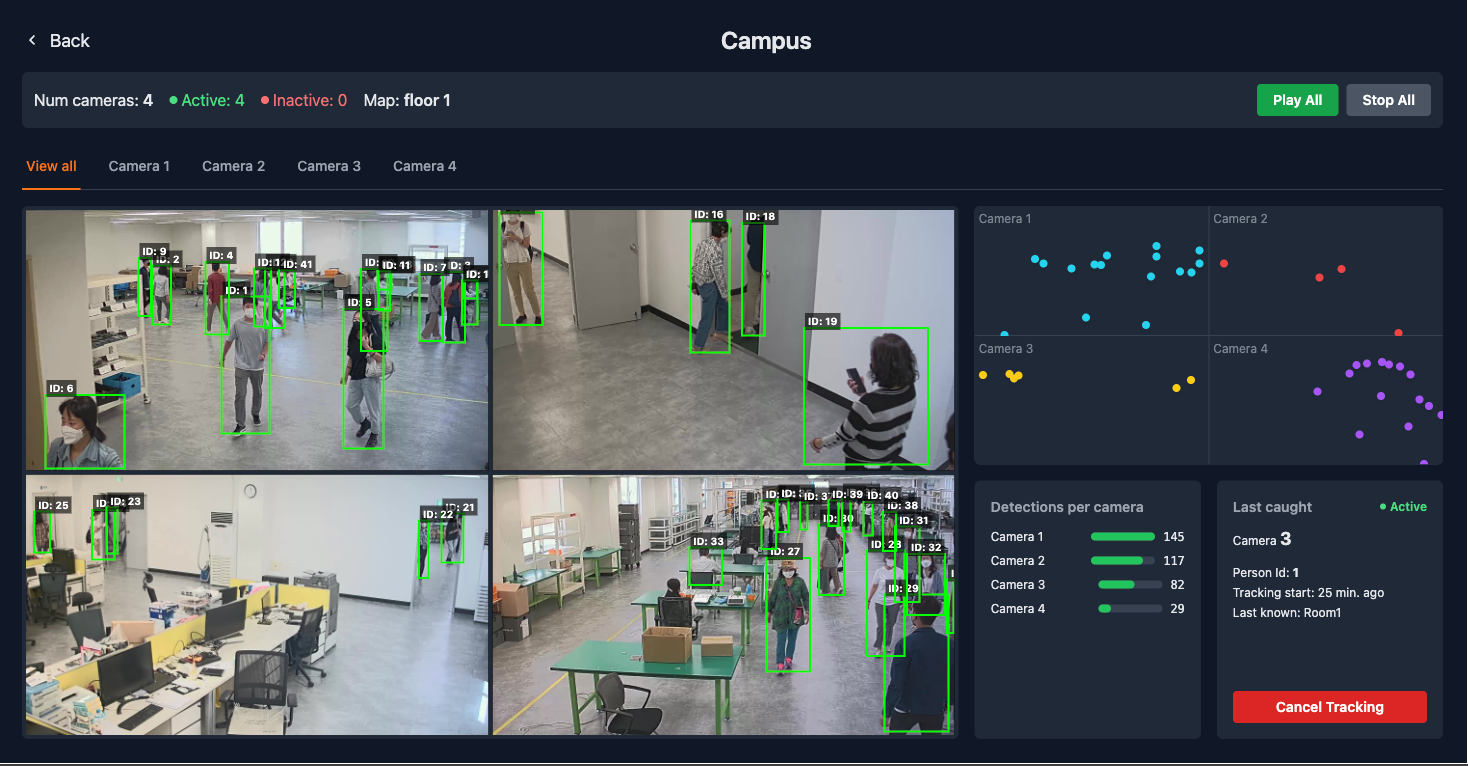
\includegraphics[width=0.9\textwidth]{assets/progress/ui_display.png}
    \caption{User interface for Multi-Camera Monitoring with AI-Driven Annotations.}
    \label{fig:ui_display}
\end{figure}
Figure \ref{fig:ui_display} showcases the implemented user interface, demonstrating the display of multi-camera video feeds annotated with AI-generated bounding boxes and an interactive map view for tracking individuals across the monitored environment.

\clearpage
\subsection*{Updated Development Plan (Gantt Chart)}
\label{subsec:progress_updated_plan}

\begin{figure}[!htb]
    \centering
    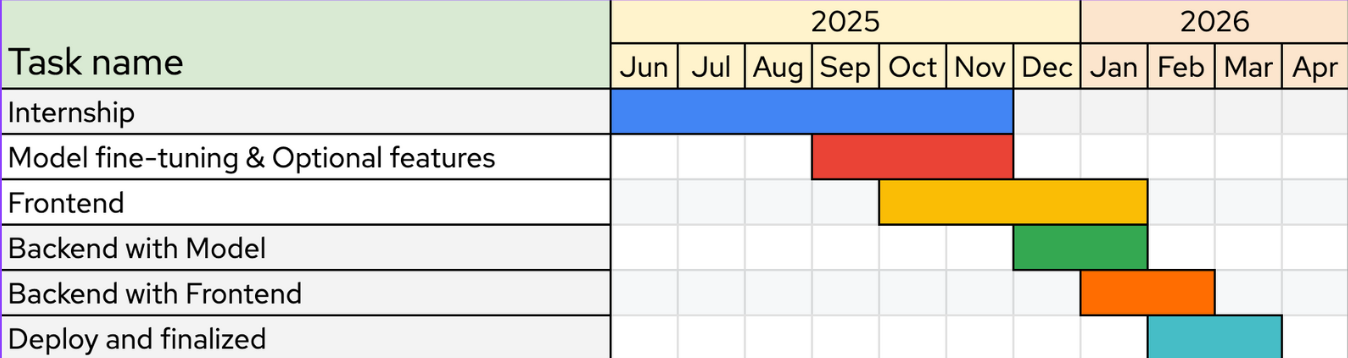
\includegraphics[width=\textwidth,height=0.8\textheight,keepaspectratio]{assets/progress/gantt_chart.png}
    \caption{Updated Development Plan (Gantt Chart)}
    \label{fig:progress_gantt_chart_placeholder}
\end{figure}

\section*{Self-Evaluation}
\label{sec:progress_self_evaluation}
The SpotOn project is currently in a strong developmental phase, with significant advancements across the MLOps pipeline, backend architecture, and frontend implementation. Progress has been steady, particularly in establishing the core functionalities for each component, such as model experimentation in MLOps, service-oriented design in the backend, and real-time data visualization in the frontend. The AI components, including fine-tuned detection models like Faster R-CNN, and the overall software architecture remain viable and well-aligned with the project's goals for multi-camera person tracking. While no major delays have been encountered, continuous integration and testing between the increasingly complex backend and frontend will be crucial moving forward. At this stage, no major strategic adjustments appear necessary, though ongoing refinement of inter-component communication protocols and performance optimization will be key focus areas.

% --- End of Progress Report Content ---